\documentclass[11pt,]{article}
\usepackage{lmodern}
\usepackage{amssymb,amsmath}
\usepackage{ifxetex,ifluatex}
\usepackage{fixltx2e} % provides \textsubscript
\ifnum 0\ifxetex 1\fi\ifluatex 1\fi=0 % if pdftex
  \usepackage[T1]{fontenc}
  \usepackage[utf8]{inputenc}
\else % if luatex or xelatex
  \ifxetex
    \usepackage{mathspec}
  \else
    \usepackage{fontspec}
  \fi
  \defaultfontfeatures{Ligatures=TeX,Scale=MatchLowercase}
\fi
% use upquote if available, for straight quotes in verbatim environments
\IfFileExists{upquote.sty}{\usepackage{upquote}}{}
% use microtype if available
\IfFileExists{microtype.sty}{%
\usepackage{microtype}
\UseMicrotypeSet[protrusion]{basicmath} % disable protrusion for tt fonts
}{}
\usepackage[margin=1in]{geometry}
\usepackage{hyperref}
\hypersetup{unicode=true,
            pdftitle={One direction? A tutorial for circular data in cognitive psychology.},
            pdfborder={0 0 0},
            breaklinks=true}
\urlstyle{same}  % don't use monospace font for urls
\usepackage{color}
\usepackage{fancyvrb}
\newcommand{\VerbBar}{|}
\newcommand{\VERB}{\Verb[commandchars=\\\{\}]}
\DefineVerbatimEnvironment{Highlighting}{Verbatim}{commandchars=\\\{\}}
% Add ',fontsize=\small' for more characters per line
\usepackage{framed}
\definecolor{shadecolor}{RGB}{248,248,248}
\newenvironment{Shaded}{\begin{snugshade}}{\end{snugshade}}
\newcommand{\AlertTok}[1]{\textcolor[rgb]{0.94,0.16,0.16}{#1}}
\newcommand{\AnnotationTok}[1]{\textcolor[rgb]{0.56,0.35,0.01}{\textbf{\textit{#1}}}}
\newcommand{\AttributeTok}[1]{\textcolor[rgb]{0.77,0.63,0.00}{#1}}
\newcommand{\BaseNTok}[1]{\textcolor[rgb]{0.00,0.00,0.81}{#1}}
\newcommand{\BuiltInTok}[1]{#1}
\newcommand{\CharTok}[1]{\textcolor[rgb]{0.31,0.60,0.02}{#1}}
\newcommand{\CommentTok}[1]{\textcolor[rgb]{0.56,0.35,0.01}{\textit{#1}}}
\newcommand{\CommentVarTok}[1]{\textcolor[rgb]{0.56,0.35,0.01}{\textbf{\textit{#1}}}}
\newcommand{\ConstantTok}[1]{\textcolor[rgb]{0.00,0.00,0.00}{#1}}
\newcommand{\ControlFlowTok}[1]{\textcolor[rgb]{0.13,0.29,0.53}{\textbf{#1}}}
\newcommand{\DataTypeTok}[1]{\textcolor[rgb]{0.13,0.29,0.53}{#1}}
\newcommand{\DecValTok}[1]{\textcolor[rgb]{0.00,0.00,0.81}{#1}}
\newcommand{\DocumentationTok}[1]{\textcolor[rgb]{0.56,0.35,0.01}{\textbf{\textit{#1}}}}
\newcommand{\ErrorTok}[1]{\textcolor[rgb]{0.64,0.00,0.00}{\textbf{#1}}}
\newcommand{\ExtensionTok}[1]{#1}
\newcommand{\FloatTok}[1]{\textcolor[rgb]{0.00,0.00,0.81}{#1}}
\newcommand{\FunctionTok}[1]{\textcolor[rgb]{0.00,0.00,0.00}{#1}}
\newcommand{\ImportTok}[1]{#1}
\newcommand{\InformationTok}[1]{\textcolor[rgb]{0.56,0.35,0.01}{\textbf{\textit{#1}}}}
\newcommand{\KeywordTok}[1]{\textcolor[rgb]{0.13,0.29,0.53}{\textbf{#1}}}
\newcommand{\NormalTok}[1]{#1}
\newcommand{\OperatorTok}[1]{\textcolor[rgb]{0.81,0.36,0.00}{\textbf{#1}}}
\newcommand{\OtherTok}[1]{\textcolor[rgb]{0.56,0.35,0.01}{#1}}
\newcommand{\PreprocessorTok}[1]{\textcolor[rgb]{0.56,0.35,0.01}{\textit{#1}}}
\newcommand{\RegionMarkerTok}[1]{#1}
\newcommand{\SpecialCharTok}[1]{\textcolor[rgb]{0.00,0.00,0.00}{#1}}
\newcommand{\SpecialStringTok}[1]{\textcolor[rgb]{0.31,0.60,0.02}{#1}}
\newcommand{\StringTok}[1]{\textcolor[rgb]{0.31,0.60,0.02}{#1}}
\newcommand{\VariableTok}[1]{\textcolor[rgb]{0.00,0.00,0.00}{#1}}
\newcommand{\VerbatimStringTok}[1]{\textcolor[rgb]{0.31,0.60,0.02}{#1}}
\newcommand{\WarningTok}[1]{\textcolor[rgb]{0.56,0.35,0.01}{\textbf{\textit{#1}}}}
\usepackage{graphicx,grffile}
\makeatletter
\def\maxwidth{\ifdim\Gin@nat@width>\linewidth\linewidth\else\Gin@nat@width\fi}
\def\maxheight{\ifdim\Gin@nat@height>\textheight\textheight\else\Gin@nat@height\fi}
\makeatother
% Scale images if necessary, so that they will not overflow the page
% margins by default, and it is still possible to overwrite the defaults
% using explicit options in \includegraphics[width, height, ...]{}
\setkeys{Gin}{width=\maxwidth,height=\maxheight,keepaspectratio}
\IfFileExists{parskip.sty}{%
\usepackage{parskip}
}{% else
\setlength{\parindent}{0pt}
\setlength{\parskip}{6pt plus 2pt minus 1pt}
}
\setlength{\emergencystretch}{3em}  % prevent overfull lines
\providecommand{\tightlist}{%
  \setlength{\itemsep}{0pt}\setlength{\parskip}{0pt}}
\setcounter{secnumdepth}{5}
% Redefines (sub)paragraphs to behave more like sections
\ifx\paragraph\undefined\else
\let\oldparagraph\paragraph
\renewcommand{\paragraph}[1]{\oldparagraph{#1}\mbox{}}
\fi
\ifx\subparagraph\undefined\else
\let\oldsubparagraph\subparagraph
\renewcommand{\subparagraph}[1]{\oldsubparagraph{#1}\mbox{}}
\fi

%%% Use protect on footnotes to avoid problems with footnotes in titles
\let\rmarkdownfootnote\footnote%
\def\footnote{\protect\rmarkdownfootnote}

%%% Change title format to be more compact
\usepackage{titling}

% Create subtitle command for use in maketitle
\newcommand{\subtitle}[1]{
  \posttitle{
    \begin{center}\large#1\end{center}
    }
}

\setlength{\droptitle}{-2em}
  \title{One direction? A tutorial for circular data in cognitive psychology.}
  \pretitle{\vspace{\droptitle}\centering\huge}
  \posttitle{\par}
  \author{Jolien Cremers\footnote{Corresponding author:
  \href{mailto:j.cremers@uu.nl}{\nolinkurl{j.cremers@uu.nl}}} \(^1\),
Irene Klugkist \(^{1,2}\)\\
\(^1\)Department of Methodology and Statistics, Utrecht University\\
\(^2\)Research methodology, Measurement and Data Analysis, Behavioural
Sciences, University of Twente}
  \preauthor{\centering\large\emph}
  \postauthor{\par}
  \date{}
  \predate{}\postdate{}


\begin{document}
\maketitle

\section{Introduction}\label{Introduction}

Circular data arises in almost all fields of research, from ecology
where data on the direction movement of animals is investigated (Rivest,
Duchesne, Nicosia, \& Fortin, 2015) to the medical sciences where
protein structure (Mardia, Taylor, \& Subramaniam, 2006) or neuronal
activity (Rutishauser, Ross, Mamelak, \& Schuman, 2010) is investigated
using periodic and thus circular measurements. The most direct examples
of circular data within the social sciences arise in cognitive and
experimental psychology. For example, in experiments on cognitive maps
the human sense of direction is investigated through asking participants
in a study to point north (Brunyé, Burte, Houck, \& Taylor, 2015) or to
walk to a certain object (Warren, Rothman, Schnapp, \& Ericson, 2017).
The closer the participants' pointing or walking direction was to the
actual north or target object, the better their sense of direction.
Other examples include the visual perception of space (Matsushima, Vaz,
Cazuza, \& Ribeiro Filho, 2014), visual working memory (Heyes, Zokaei,
\& Husain, 2016) and sensorimotor synchronization in music making
(Kirschner \& Tomasello, 2009).

However, despite the fact that circular data is being collected in
different areas of cognitive and experimental psychology, the knowledge
of this type of data is not well-spread. Circular data is fundamentally
different from linear data due to its periodic nature. On the circle,
measurements at 0\(^\circ\) and 360\(^\circ\) represent the same
direction whereas on a linear scale they would be located at opposite
ends of a scale. For this reason circular data require specific analysis
methods. Some less technical textbooks on analysis methods for circular
data have been written (Batschelet, 1981; Fisher, 1995; Pewsey,
Neuhäuser, \& Ruxton, 2013). However these works are not part of the
`standard' texts on statistical analysis in psychology or the social
sciences in general nor are they very well known amongst social
scientific researchers.

Therefore, this paper aims at giving a tutorial in working with and
analysing circular data to researchers in congintive psychology and the
social sciencesin general. The main goal of this tutorial is to explain
how to inspect and analyse your data when the outcome variable is
circular. We will discuss data inspection, model fit, estimation and
hypothesis testing in general linear models (GLM) and mixed-effects
models. In this tutorial we decide to mainly focus on one particular
approach to the analysis of circular data, the embedding approach. We do
so for the flexibility of this approach and the resulting variety in
types of models that have already been outlined in the literature on
circular data for this approach. Note that for an optimal understanding
of the paper, the reader should ideally have some knowledge on \verb|R|
and on multiple regression and mixed-effects models in the linear
setting. The reader does not need to be familiar with circular data.

The structure of the tutorial is such that the reader is guided by two
examples throughout the paper. One is an example for an ANOVA model and
the other for a mixed-effects model. First however, we give a short
introduction to circular data in general in Section \ref{circdat}. Next,
in Section \ref{DataInspection}, we introduce the ANOVA example after
which descriptive methods for circular data are explained through a
section on data inspection for this example. After that we will continue
with an analysis of the example datasets. First we analyse the ANOVA
dataset using a method for circular GLM and give interpretation
guidelines for this model in Section \ref{RegModel}. Next, in Section
\ref{MEModel} we will introduce and analyse the mixed-effects example
data. Again, we analyse this data and include guidelines for
interpretation. The analyses of both datasets, the ANOVA and
mixed-effects dataset, are performed using the package \verb|bpnreg|.
For both models we use, the GLM and the mixed-effects model for a
circular outcome we write a short technical section (sections
\ref{EmbeddingApproach} and \ref{embeddingME}) in which the mathematical
details of the respective models are given. Lastly, a summary of the
paper and additional references to literature on other models for
circular data are given in Section \ref{conclusion}.

\section{Circular data}\label{circdat}

In the introduction we have briefly mentioned that circular data is data
that has a periodic nature. The most intuitive form of circular data
comes in the form of directions on a compass. For example, a participant
in an experiment could be instructed to move or point to a certain
target. We can then measure the direction, North, South, East or West on
a scale from 0 to 360 degrees. A plot of such measurements for several
participants is shown in Figure \ref{plotdir}. In this plot we can
easily see the periodicity of the data, 0\(^\circ\) represents the same
datapoint as 360\(^\circ\). Furthermore, we can see what happens if we
would treat this data in the `usual' linear way. Participants that moved
North-East have a score of 45\(^\circ\) and participants that moves
South-East have a score of 315\(^\circ\). On the circle we can see that
this is only 90\(^\circ\) apart, while on a linear scale it is much
further apart at 315\(^\circ\) - 45\(^\circ\) = 270\(^\circ\). More
importantly however, there is a difference between the circular and
linear means for this data. In Figure \ref{plotdir} we see that the
circular mean direction is 0\(^\circ\). The linear mean however is
180\(^\circ\) and is opposite to the actual mean direction of the data.
Clearly, a linear treatment of the data in Figure \ref{plotdir} can lead
to incorrect conclusions.

\begin{figure}
        \centering

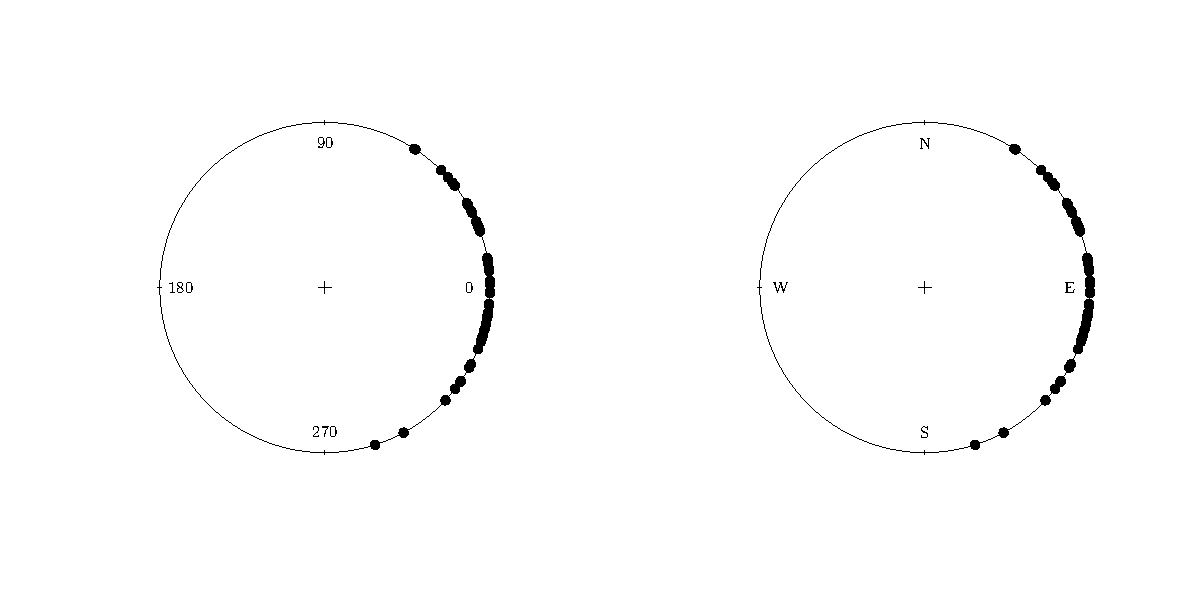
\includegraphics[width=\textwidth]{plotdir.pdf}

         \caption{Data from participants in an experiment that were instructed to move East. The plot on the left shows the data on a 0$^\circ$ - 360$^\circ$ scale. The plot on the right shows the data on the compass.}
        \label{plotdir}
\end{figure}

Clock times are another type of circular data. We might for instance be
interested at what time of day a certain event takes place, e.g.~the
time of day at which positive affect is highest. Figure \ref{plothour}
shows data the time of day at which positive affect is highest for two
groups of participants, e.g. two groups of psychiatrical patients who
are being treated for depression at different clinics. From the plots we
clearly see that the peak of positive affect for the two groups is at
roughly the same time of day, one slightly before 12 pm and one slighly
after. However, if we were to analyze this data using standard
statistics for linear data and we would compare the means of the two
groups, 11 pm and 1 am we would reach a completely different conclusion.
The two means are namely at the two opposite ends of a linear scale from
00.00 am to 12.00 pm, and we would counclude that the time of day at
which positive affect is highest is different for the two groups.

\begin{figure}
        \centering

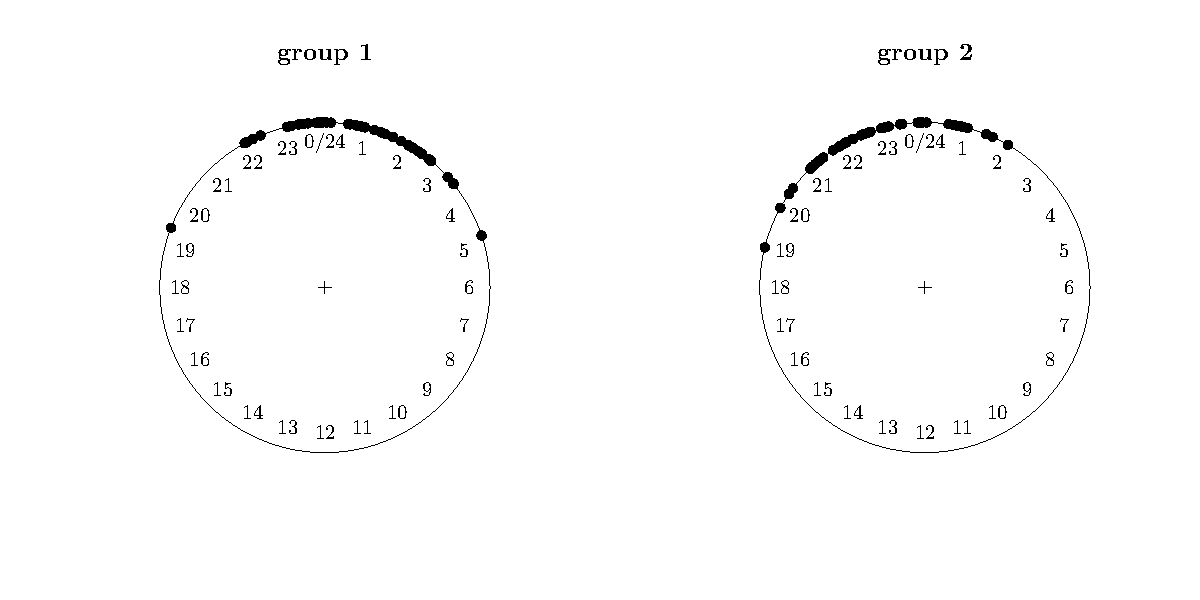
\includegraphics[width=\textwidth]{plothour.pdf}

         \caption{Data for the hour at which positive affect is highest for two groups of
psychiatrical patients who are being treated for depression at different
clinics.}
        \label{plothour}
\end{figure}

The two examples of circular data that we have just given illustrate why
it is important to treat circular data differently from linear data.
This goes both for describing your data, e.g.~computing circular means
as well as analyzing them, e.g.~testing whether the circular means of
two groups differ. In the next section we will introduce an example
dataset on which we will show several ways to inspect and compute
descriptive measures for circular data.

\section{Inspecting your data}\label{DataInspection}

Before any statistical analysis it is wise to inspect your data. In this
section we will outline a basic way to do so using the \verb|R| packages
\verb|bpnreg| and \verb|circular| (Agostinelli \& Lund, 2013). We will
illustrate this for an example dataset, the motor resonance data,
introduced below.

\subsection{The motor resonance data}\label{regressionexample}

In this section we introduce data from an article by Puglisi et al.
(2017) on human motor resonance. From now on we will call this data the
motor resonance data. Motor resonance is a response in the brain in the
primary motor cortex and spinal circuits that is caused by observation
of others' actions. In their research Puglisi et al. (2017) conduct an
experiment in which `observers' are asked to either look at the movement
of a hand of a `mover' or at another other object in order to evaluate
the role of attention in motor resonant response. The experiment has
three conditions: the `explicit observation' condition (n = 14), where
observers are explicitly instructed to observe the hand, the
`semi-implicit observation' condition (n = 14) where the observers have
to perform a task that requires the implicit observation of the hand of
the mover and the `implicit observation' condition (n = 14), where
observers have to perform a task that is independent of the observation
of the hand of the mover. The idea of motor resonance is that the
`observer' starts moving his or her hand in the same manner as the
`mover' because he or she is implicitly or explicitly observing the hand
of the `mover'. This is the resonant response. This resonant response is
hypothesized to be strongest and more synchronized with the hand
movement of the mover in the explicit condition and smallest in the
implicit condition. In each condition the hand movements of the
observers were measured and the phase difference between movement of the
the observers' hand and the hand of the mover was calculated. This phase
difference is a measurement of the strength of the resonant response and
a circular variable. It can thus be described and analyzed using
circular statistics. In addition to the phase difference the average
amplitute of the hand movement of the observer was computed. Note that
in the original article there was also a baseline condition (n=14)
without a mover. Instead, observers had to look at an inanimate object
that moves in an identical manner to the hand of the mover in other
conditions. The baseline condition is however not included in the
example data since no resonant response was observerd in the observers'
hand according to the original research.

The motor resonance data can be found in the package \verb|bpnreg| as
the dataframe \verb|Motor|. \verb|Motor| is a dataframe with 42 rows and
7 variables. The variable \verb|Cond| indicates the condition (explicit,
semi-implicit and implicit) a participant was placed in, the
\verb|AvAmp| variable contains the average amplitude, and that the
\verb|PhaseDiff| and \verb|Phaserad| variables contain the measured
phase difference between `observer' and `mover' in degrees and radians
respectively.

\subsection{Plots for circular data}\label{Plots}

The main question of interest for the motor resonance data is whether
the phase difference between the three experimental conditions differs.
To be more precise whether there is a smaller phase difference in the
explicit condition than in the other two. Differences that are observed
in the phase difference are interpreted as differences in the strength
of the resonant response (Puglisi et al., 2017). A smaller phase
difference indicates a stronger an more synchronized resonant response.
A first step to investigating the question of interest is plotting the
phase differences of the three conditions. We can do so using the
package \verb|circular|.

\begin{figure}
        \centering

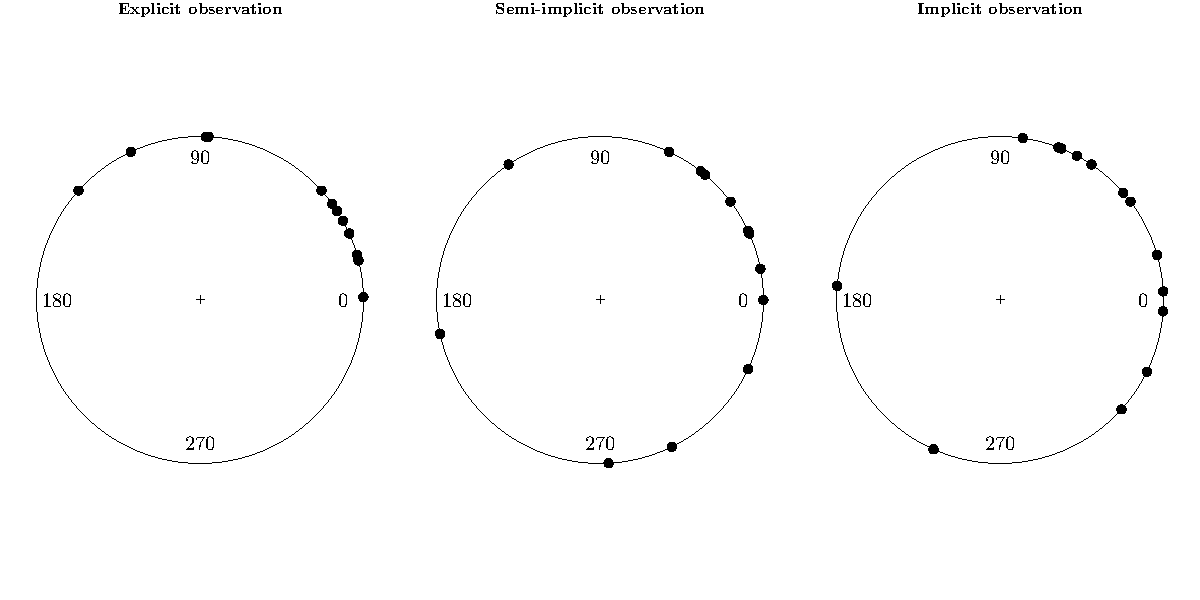
\includegraphics[width=\textwidth]{plot_motorresonance.pdf}

         \caption{Plots of the phase differences for each condition of the motor resonance data.}
        \label{motorplot}
\end{figure}

Figure \ref{motorplot} shows the plots of the phase differences of each
condition. We see that the phase differences in the explicit condition
are much less spread out on the circle than the phase differences in the
other two conditions. Also the average phase differences seem to differ
between the conditions. In the next section we show measures for the
mean and variance of a sample of circular data.

\subsection{Circular mean, resultant length and variance}\label{MeanVariance}

\begin{table}
\centering
\caption{Descriptives for the motor resonance data with mean direction ($\bar{\theta}$), mean resultant length ($\bar{R}$), circular variance ($V_m$) and circular standard deviation ($v$) of the phase difference for each condition.} 
\begin{tabular}{lrrrr}
  \hline\noalign{\smallskip}
Phase difference & $\bar{\theta}$ & $\bar{R}$ & $V_m$ & $v$ \\ \hline\noalign{\smallskip}
explicit         & 49.55$^{\circ}$ & 0.77 & 0.23 & 41.39$^{\circ}$\\ 
semi.implicit    & 18.45$^{\circ}$ & 0.54 & 0.46 & 63.82$^{\circ}$\\
implicit         & 31.94$^{\circ}$ & 0.56 & 0.44 & 61.72$^{\circ}$\\
   \hline
\end{tabular}
\label{TableDescriptives}
\end{table}

Table \ref{TableDescriptives} shows descriptives for the motor resonance
data. For each group, the table contains a circular mean and a mean
resultant length of the phase difference. The circular population mean,
\(\mu\), indicates the average direction of a certain variable in the
population. The population mean resultant length, \(\rho\), is a
statistic between 0 and 1 that gives us information on the spread of a
circular variable in the population. It is interpreted as a precision
measure where 0 means that the spread is large and 1 means that all data
are concentrated at a single value. Sample statistics for these values
are \(\bar{\theta}\) for the mean and \(\bar{R}\) for the mean resultant
length. Fisher (1995) explains how to compute these two statistics.

Graphically we can illustrate their computation as shown in Figure
\ref{meanrbarplot}. On the left side of this figure we see two sets of
circular data. We represent represent a circular datapoint as a vector
composed of the cosine and sine of the datapoint instead of one value a
measure in degrees (or radians). E.g. for a score of 90\(^\circ\) we
have the following vector \((\cos(90^\circ), \sin(90^\circ))\). The
solid vectors in Figure \ref{meanbarplot} each represent one circular
datapoint. To compute the mean directions and resultant lengths for the
datasets on the left we place the vectors head to toe, as in the right
side of Figure \ref{meanrbarplot}. We then connect the toe of the first
vector to the head of the last vector. This results in the dotted
vectors on the right side of Figure \ref{meanrbarplot}. The direction of
the dotted vector is the mean direction, \(\bar{\theta}\) of the vectors
from which it was created. The length of the dotted vector is the
resultant length. The mean resultant length, \(\bar{R}\) is the length
of this vector divided by the amount of vectors from which it was
created. In Figure \ref{meanrbarplot} we see that the data in the bottom
left figure are much more concentrated on the circle than the data in
the upper left figure. This translates to the resultant length in the
bottom right being larger than the resultant length (length of the
dotted vector) in the upper left.

\begin{figure}
        \centering

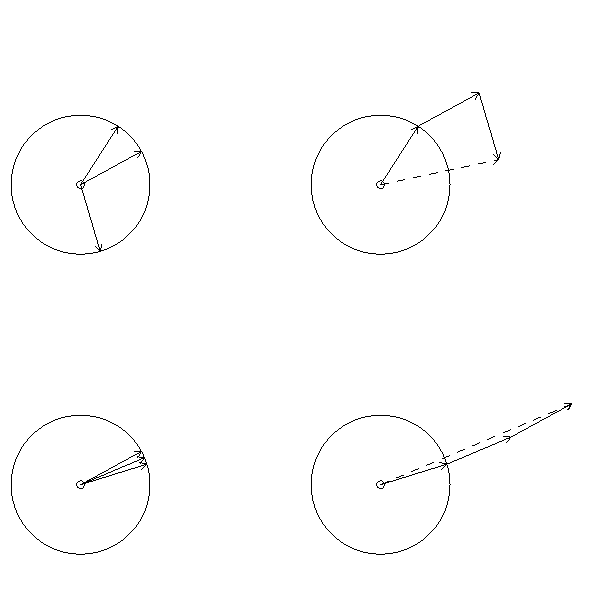
\includegraphics[width=\textwidth]{meanrbar.pdf}

         \caption{The computation of a circular mean and (mean) resultant length (right) for two sets of circular data (left). The solid lines are vectors representing the circular datapoints. The direction of the dotted vector is the mean direction and the length of the dotted vector is the resultant length.}
        \label{meanrbarplot}
\end{figure}

In Table \ref{TableDescriptives} we see that in the motor resonance data
the circular mean of the phase difference for the explicit observation
condition is highest with 49.55\(^{\circ}\). The mean phase differences
for the semi-implicit and implicit observation conditions are lower at
18.45\(^{\circ}\) and 31.94\(^{\circ}\). Moreover, the mean resultant
lengths of the three groups differ. The phase differences of the
individuals in the explicit observation condition are most concentrated
with \(\bar{R} = 0.77\). The phase differences differ more between the
individuals in the semi-implicit and implicit observation conditions
where the spread is larger at \(\bar{R}\)'s of 0.54 and 0.56
respectively.

Table \ref{TableDescriptives} also shows a circular variance and
standard deviation. The sample value, \(V_m\) for the circular variance
is defined as \(1-\bar{R}\). Its interpretation is exactly opposite to
the interpretation of the mean resultant length. A variance of one means
that a variable has a very large spread and a variance of 0 means that
all data are concentrated at one point. Note that unlike a linear
variance the circular variance is bounded between 0 and 1. A sample
circular standard deviation, \(v\), can also be computed (Fisher, 1995).

We have seen that both the average phase difference and variances of the
phase difference seem to be different for the three conditions in the
motor resonance data. To test whether these differences in circular
means also exist in the population, we can use a a projected normal
regression model. In the next section we will introduce this model and
fit it to the motor resonance data.

\section{A general linear model with a circular outcome}\label{RegModel}

In this section we will introduce a projected normal circular regression
model. This model falls within the embedding approach to circular data.
Note that because it is a regression model we can also fit AN(C)OVA type
models with it, we can thus refer to it as a circular GLM. As noted in
the introduction, we choose to focus on a model from the embedding
approach since this approach is quite flexible in the sense that it is
relatively easy to translate models that exist for linear data to the
circular case. We will first outline the theoretical background to the
projected normal circular regression model and the embedding approach
after which we will continue to fit an ANOVA to the motor resonance
data. At the end of this section we will shortly consider two different
methods for circular ANOVA.

\subsection{The embedding approach to circular data}\label{EmbeddingApproach}

In the previous section, at the computation of the circular mean, we
have seen that a circular variable \(\theta\), e.g.~the phase difference
in the motor resonance data, can be expressed as a unit vector
\(\boldsymbol{u}\) composed of the sine and the cosine of an angle
\(\boldsymbol{u} = (\cos\theta, \sin\theta)\). If we translate this to
bivariate real space the cosine is the x-component and the sine is the
y-component of an angle. In the embedding approach we assume that the
circular variable \(\boldsymbol{u}\) origins from the following
relation:

\begin{equation}\label{embedding}
 \boldsymbol{u} = \boldsymbol{y} / r 
\end{equation}

We assume that \(\boldsymbol{u}\) can be multiplied by a positive linear
variable \(r\), \(0 < r \leq \infty\), to obtain a bivariate normal
variable \(\boldsymbol{y}\). Note that in a real dataset with sample
size \(n\) we have a set of vectors \(\boldsymbol{u}_{i}\), one for each
person \(i = 1, \dots, n\). This also means that there is an underlying
vector \(\boldsymbol{y}_{i}\) and value \(r_{i}\) for each person in our
dataset. Figure \ref{projectingplot} depicts this relation between
\(\boldsymbol{u}_{i}\) and \(\boldsymbol{y}_{i}\).

\begin{figure}
        \centering

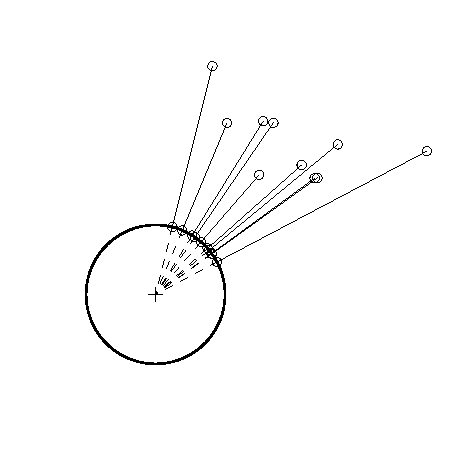
\includegraphics[width=\textwidth]{plotprojecting.pdf}
       
        \caption{A set of datapoints in bivariate space $\boldsymbol{y}_i$ projected onto the circle to produce         a set of datapoints $\boldsymbol{u}_i$. The lines connecting the datapoints to the origin of the circle         represent $r_i$.}
        
        \label{projectingplot}
        
\end{figure}

The projected normal regression model is introduced by Presnell,
Morrison, \& Littell (1998). This model makes use of the embedding
approach to circular data. The idea behind the embedding approach is to
not conduct inference on the circular variable \(\theta\) directly but
to indirectly conduct inference on the underlying bivariate normal data
in \(\boldsymbol{y}\). This makes the embedding approach a flexible
approach to circular data as many different and complex types of models
already exist for bivariate normal data. However, both the vector
\(\boldsymbol{y}\) and value \(r\) are quantities that can not be
obtained directly from \(\theta\). The estimation of these objects is a
missing data problem. The solution for this missing data problem used in
this paper relies on Bayesian estimation. More details on this Bayesian
method are outlined by Nuñez-Antonio, Gutiérrez-Peña, \& Escarela (2011)
and Cremers, Mulder, \& Klugkist (2018) for regression models.

Assuming that \(\boldsymbol{y}\) has a bivariate normal distribution,
the relation in Equation \ref{embedding} implies that \(\theta\) has a
projected normal distribution. The projected normal (PN) distribution
for the cicular outcome \(\theta\) is expressed as:

\begin{equation}\label{PN} PN(\theta \mid \boldsymbol{\mu}, \boldsymbol{I})  =
\frac{1}{2 \pi} e^{-\frac{1}{2}\vert \vert \boldsymbol\mu \vert \vert ^ 2}
\left[1+\frac{\boldsymbol{u}^t\boldsymbol\mu\Phi(\boldsymbol{u}^t\boldsymbol\mu)}{\phi(\boldsymbol{u}^t\boldsymbol\mu)}\right],
\end{equation}

where \(\theta\) is measured in radians \(-\pi \leq \theta < \pi\),
\(\boldsymbol{\mu} = (\mu_{1}, \mu_{2})^{t} \in \mathbb{R}^2\) is the
mean vector of the distribution, the variance-covariance matrix
\(\boldsymbol{I}\) is an identity matrix, and
\(\boldsymbol{u}^{t} = (\cos \theta, \sin \theta)\). The terms
\(\Phi(\cdot)\) and \(\phi(\cdot)\) denote the cumulative distribution
function and the probability density function of the standard normal
distribution respectively. When fitting a model using the PN
distribution we are interested in modelling its mean vector
\(\boldsymbol{\mu}\).

In regression models, \(\boldsymbol{\mu}\) has a regression structure.
In a multiple regression model this is specified as follows:

\begin{equation}\label{regression}
\boldsymbol{\mu}_{i} = \begin{pmatrix}
  \mu_{i}^{I}  \vspace{0.2cm}  \\
\mu_{i}^{II}
 \end{pmatrix}=\begin{pmatrix}
  (\boldsymbol{\beta}^{I})^{t}\boldsymbol{x}_{i}^{I} \vspace{0.2cm}  \\
  (\boldsymbol{\beta}^{II})^{t}\boldsymbol{x}_{i}^{II} 
 \end{pmatrix},
\end{equation}

where \(I\) and \(II\), the two components, are the x and y axis of the
Cartesian plane, \(i = 1, \dots, n\), \(\boldsymbol{x}_{i}\) is a vector
of predictor values for individual \(i\) and each \(\boldsymbol{\beta}\)
is a vector with intercept and regression coefficients. To be able to
estimate an intercept, the first component of \(\boldsymbol{x}_{i}\)
equals 1. Note that the vectors \(\boldsymbol{x}_{i}\) are allowed to
differ for the two components \(I\) and \(II\). In the next section we
will fit this type of model to the motor resonance data.

In terms of interpretation of the circular effect of a variable the two
component structure in (\ref{regression}) poses a problem. The two
components do not necessarily have a useful interpretation for each type
of circular data, e.g.~we cannot talk of a 12 o'clock and 6 o'clock axis
in Figure \ref{plothour}. Cremers et al. (2018) outline how this problem
can be overcome and introduce new interpretation tools in PN multiple
regression models that transform the effects on the two components to an
effect on the circle. In this tutorial we will use these tools and
interpret coefficients of a circular effect and not the coefficients for
each of the components.

\subsection{Fitting an ANOVA model to the motor resonance data}\label{RegModelMotor}

In this section we will fit a circular ANOVA model to the motor
resonance data using the package \verb|bpnreg|. Note that the model from
this package is in fact a regression model that we can speficy in such a
way that it is mathematically equivalent to an ANOVA. First we will give
the details on this model and subsequently we will discuss and interpret
the results.

\subsubsection{Fitting the model}\label{fitMotor}

To investigate the effect of condition on the phase difference we
specify the prediction equation for the mean vector in the projected
normal regression model as follows:

\begin{equation}\label{regressionmotor}
\boldsymbol{\mu}_{i} = \begin{pmatrix}
  \mu_{i}^{I}  \vspace{0.2cm}  \\
\mu_{i}^{II}
 \end{pmatrix}=\begin{pmatrix}
  \beta_{0}^{I} +  \beta_{1}^{I}\text{semi.implicit}_{i}+  \beta_{2}^{I}\text{implicit}_{i} \vspace{0.2cm}  \\
  \beta_{0}^{II} +  \beta_{1}^{II}\text{semi.implicit}_{i}+  \beta_{2}^{II}\text{implicit}_{i}  
 \end{pmatrix},
\end{equation}

where the variables semi.implicit and implicit are dummy variables
indicating condition membership, \(\beta_{0}^{I}\) and
\(\beta_{0}^{II}\) are the intercepts and \(\beta_{1}^{I}\),
\(\beta_{2}^{I}\), \(\beta_{1}^{II}\) and \(\beta_{2}^{II}\) are the
regression coefficients of the model. Note that in this model we take
the explicit observation condition as the reference condition. When we
translate this to the ANOVA context, the intercepts, \(\beta_{0}^{I}\)
and \(\beta_{0}^{II}\), represent the mean for the explicit condition,
\(\beta_{0}^{I} + \beta_{1}^{I}\) and
\(\beta_{0}^{II} + \beta_{1}^{II}\) are expressions for the mean of the
semi-implicit condition and \(\beta_{0}^{I} + \beta_{2}^{I}\) and
\(\beta_{0}^{II} + \beta_{2}^{II}\) are expressions for the mean of the
implicit condition.

We use the package \verb|bpnreg| to fit the model. Because this is a
Bayesian method we have to specify some parameters for the MCMC sampler
that estimates the parameters of the model. MCMC methods are iterative
and we thus need to specify the number of iterations that we want to
run. We choose a relatively high number of the output iterations
(\verb|its = 10000|) to make sure that the sampler converges and that we
don't need to run it again in case it did not. We choose the burn-in
period to consist of 100 iterations (\verb|burn = 100|). This means that
we throw away the first 100 iterations to make sure that the iterations
we keep are those at which the sampler has reached its equilibrium. We
also choose the lag, that is how many iterations we want to keep, in
this case every third iteration (\verb|n.lag = 3|). We set a lag to
prevent possible auto-correlation between the parameter estimates. In
the next section we will elaborate further on how to check convergence
and choose these MCMC parameters wisely. But first, we fit the model:

\begin{Shaded}
\begin{Highlighting}[]
\NormalTok{fit.Motor <-}\StringTok{ }\KeywordTok{bpnr}\NormalTok{(}\DataTypeTok{pred.I =}\NormalTok{ Phaserad }\OperatorTok{~}\StringTok{ }\DecValTok{1} \OperatorTok{+}\StringTok{ }\NormalTok{Cond, }\DataTypeTok{data =}\NormalTok{ Motor,}
                  \DataTypeTok{its =} \DecValTok{10000}\NormalTok{, }\DataTypeTok{burn =} \DecValTok{100}\NormalTok{, }\DataTypeTok{n.lag =} \DecValTok{3}\NormalTok{, }\DataTypeTok{seed =} \DecValTok{101}\NormalTok{)}
\end{Highlighting}
\end{Shaded}

\subsubsection{Convergence}

In a Bayesian model that uses MCMC sampling for estimation we always
have to assess convergence of the MCMC chain for all parameters in the
model. A traceplot is one way to assess the convergence of a parameter.
As an illustration we will show the traceplot for the MCMC chains for
one of the parameters of the model.

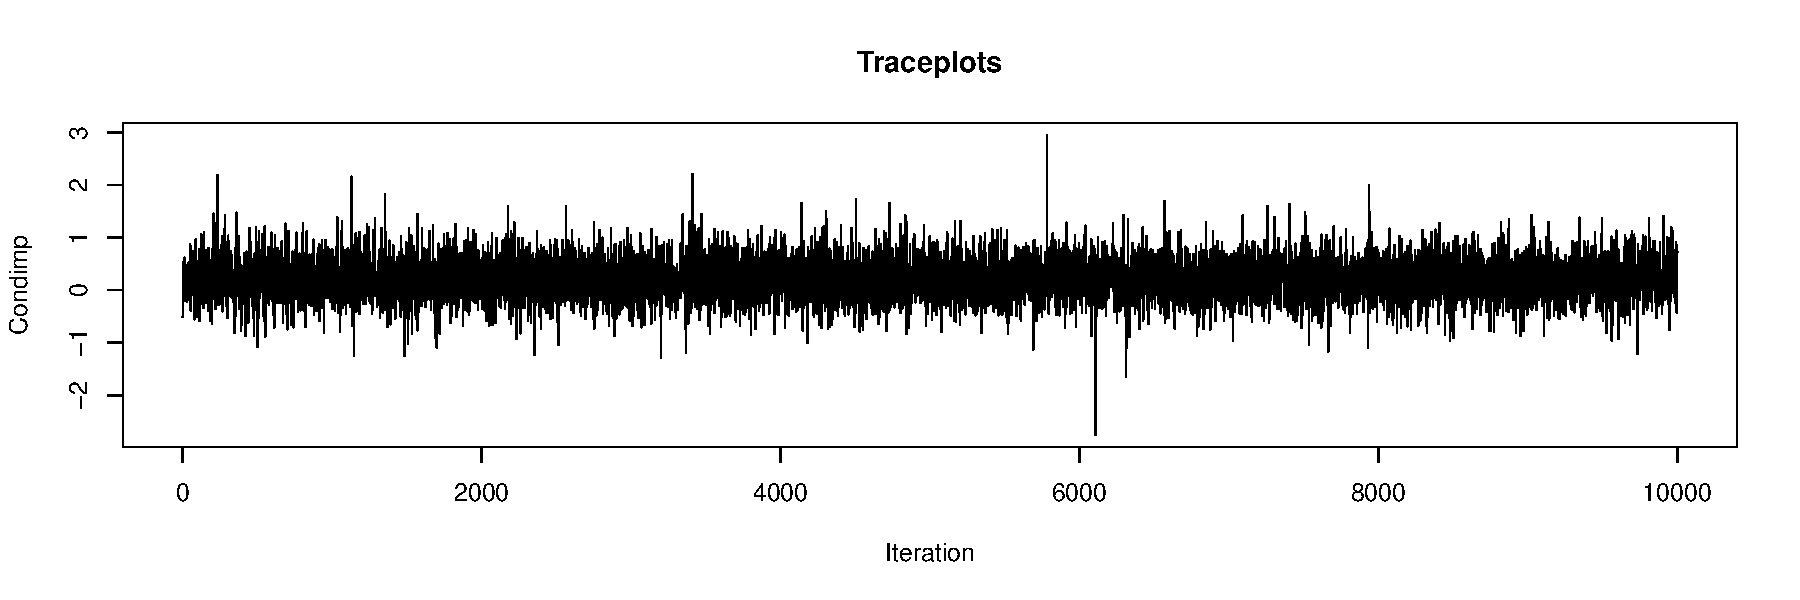
\includegraphics{ManuscriptMarkdownV2_files/figure-latex/unnamed-chunk-6-1.pdf}

From the previous traceplots we may conclude that the MCMC chain
converged within 10000 iterations and a burn-in of 100. The plot looks
like a `fat-caterpillar' meaning that the chain has reached an
equilibrium around a particular value. In case an MCMC chain does not
converge we could have add more iterations, a larger \verb|n.lag| or
more burn-in iterations. We can also evaluate other convergence
diagnostics. The focus of this paper however does not lie on Bayesian
data analysis and therefore we refer to other works, e.g. Gelman et al.
(2014), for more information on assessing convergence.

\subsubsection{Results}\label{ResMR}

To answer the question whether the conditions of the motor resonance
data differ in their phase difference we investigate the estimated
circular regression coefficients. In Cremers et al. (2018) it is
explained how to obtain circular regression coefficients for continuous
variables and how to interpret them. However, because there are no
continuous variables in the model we only get estimates for the circular
means of the three conditions in the data. Because we use a Bayesian
method we in fact get the posterior distributions of these means.
Philosophically, in Bayesian statistics each parameter is said to have
its own distribution. The posterior distribution is the result of the
prior knowledge we have about a parameter before conducting a study,
formalized as a `prior'
distribution\footnote{In this paper we choose non-informative priors for
the parameters.} and the information that lies in the data obtained from
a study, formalized as the likelihood. The fact that we obtain the
distribution of a parameter is convenient for inference purposes since
this means that we do not just have a point estimate of a parameter (the
mean or mode of the posterior distribution) but we also automatically
get an uncertainty estimates (the standard deviation of the posterior
distribution).\footnote{For more background
on Bayesian statistics see e.g. Gelman et.al. (2014).}

\begin{table}
\centering
\caption{Descriptives of the posterior distributions of the circular means of the phase diferencefor the three conditions of the motor resonance data.} 
\begin{tabular}{llllll}
  \hline\noalign{\smallskip}
Condition & Mode & Mean & sd & LB HPD & UB HPD\\ \hline\noalign{\smallskip}
explicit & 42.70$^\circ$ & 45.56$^\circ$ & 11.67$^\circ$ & 22.26$^\circ$ & 67.99$^\circ$\\
semi-implicit & 21.08$^\circ$ & 19.40$^\circ$ & 18.36$^\circ$ & -18.27$^\circ$ & 55.22$^\circ$\\
implicit & 37.22$^\circ$ & 33.47$^\circ$ & 17.77$^\circ$ & -2.25$^\circ$ & 68.22$^\circ$\\
   \hline
\end{tabular}
\label{TableresMRmean}
\end{table}

Summary statistics for the posterior distributions of the circular means
for each condition are shown in Table \ref{TableresMRmean}. This table
shows the posterior mean, mode, standard deviation (sd) and the lower
and upper bound of the 95\(\%\) highest posterior density interval
(HPD). The standard deviation of a posterior is an estimate for the
standard error of the parameter. The HPD interval is the smallest
interval in which 95\(\%\) of the posterior mass is located. In terms of
interpretation, it is different from a frequentist confidence interval
since HPD intervals allow for probability statements. For example, if
the 95\(\%\) HPD interval for a parameter \(\mu\) runs from 2 to 4 we
can say that the probability that \(\mu\) lies between 2 and 4 is 0.95.

HPD intervals can also be used to test whether a parameter is different
from a certain value or whether two parameter estimates are different.
In Table \ref{TableresMRmean} we see that the HPD intervals of the
circular means for the three conditions in the motor resonance data
overlap. The cicular mean of the phase difference is estimated at
47.70\(^\circ\) (22.26\(^\circ\); 67.99\(^\circ\)) for the explicit
condition, 37.22\(^\circ\) (-2.25\(^\circ\); 68.22\(^\circ\)) for the
implicit condition and 21.08\(^\circ\) (-18.27\(^\circ\);
55.22\(^\circ\)) for the semi-implicit condition. We thus conclude that
the circular means for the three conditions do not differ and that there
is no effect of condition on the average phase difference.
\textcolor{red}{Ook de varianties van de drie groepen
vergelijken?}

\subsection{Other approaches to circular ANOVA}\label{otheranova}

In the previous section we have tested whether the mean phase
differences of the three conditions differ in the population using a
Bayesian projected normal regression model. We can also do this using a
frequentist ANOVA for circular data that tests the hypothesis
\(H_0: \mu_{explicit} = \mu_{semi-implicit} = \mu_{implicit}\). One of
such tests is the Watson-Williams test. This test can be perfomed using
the function \verb|watson.williams.test| in the \verb|circular| package
and is similar to an ANOVA for linear data interpretation-wise. As in
the projected normal regression model we conclude from this test that
the average phase differences of the three conditions are not
significantly different: F(2, 39) = 1.02, p \textgreater{} 0.05.

As in ANOVA models for linear data, we have to meet a set of assumptions
for this test to be valid. Firstly, the samples from the different
conditions are assumed to be von-Mises distributed in the
Watson-Williams test. Secondly, the samples are assumed to have the same
circular variance. The von-Mises distribution is a type of distribution
for circular data, it is unimodal with mean \(\mu\) and concentration
\(\kappa\). The assumption of homogeneity of variance is tested within
the \verb|watson.williams.test| function itself. The assumption of
von-Misesness can be tested using e.g.~the Watson's goodness of fit test
for the von Mises distribution. If we perform this test on the phase
differences of the three subgroups we conclude that only the phase
differences from the \verb|semi.implicit| and the \verb|implicit|
condition are von-Mises distributed (\(H_0\) is not rejected). This
means that it is not completely valid to perform the Watson-Williams
test on the motor resonance data. In addition, the Watson-Williams test
does not allow for the addition of covariates and thus cannot estimate
AN(C)OVA models.

Another method that we can use is a Bayesian circular GLM that falls
within the intrinsic approach. The intrinsic approach to circular data
differs from the embedding approach in the sense that it uses
distributions that are directly defined on the circle instead of
projecting distributions in bivariate linear space onto the circle. The
Watson-Williams test is thus also a method that falls within the
intrinsic approach. The Bayesian circular GLM can be fit using the
package \verb|circglmbayes|. Note that because it is a GLM this method
can also fit ANCOVA and regression models.
\textcolor{red}{Dit model ook fitten?}

\section{Mixed-Effects models with a circular outcome}\label{MEModel}

In this section we will introduce the circular mixed-effects model. We
will first introduce a new dataset, the cognitive maps data, and give
descriptive statistics. Then, we will shortly outline the theoretical
background to the mixed-effects model and fit it to the cognitive maps
data.

\subsection{The cognitive maps data}\label{CogMap}

The cognitive maps data is a subset of data from a study by Warren et
al. (2017) on the geometry of humans' knowledge of navigation space. In
their study Warren et al. (2017) amongst others conduct an experiment in
which a total of 20 participants used virtual reality headsets to
navigate through one of two a virtual mazes. The navigation task
consisted of walking from a start object to a target object. In a
training phase they had learned to navigate between different pairs of
start and target objects in one of two versions of the maze. The number
of trials each participant completed in this training phase was
recorded. In the test phase of the experiment participants first walked
to a start object. When they had reached this object the maze
dissappeared and only a ``textured groundplane'' of the maze remained
visible. The participants then turned toward the location of the target
object that they had remembered during the training phase and started to
walk toward the target. The angular difference between the initial
walking direction of a participant from the start object and the
location of the target object, that is, the angular error, was recorded
as an outcome variable in the experiment.

The type of maze is a between-subjects factor, participants either had
to navigate through a `Euclidean' maze or a `non-Euclidean' maze. The
Euclidean maze is the standard maze and is a maze just as we know it in
the real world. The other version of the maze, the non-Euclidean maze,
has exactly the same layout as the standard maze but it has virtual
features that do not exist in reality. It namely contains wormholes by
which participants can be `teleported' from one place in the maze to
another.

In the test phase of the experiment all participants had to complete 8
trials. In each of these trials participants had to walk to a specific
target object. A within-subjects factor is the type of target object.
Pairs of start and target objects were of two types: probe and standard.
The probe objects were located near the entrance and exit of a wormhole
in the non-Euclidean maze whereas the standard objects were located at
some distance from the wormholes. For each of these two types of objects
participants had to find 4 different targets resulting in a total of 8
trials per participant.

For this experiment we could be interested in the question whether the
participants in the non-Euclidean maze make use of the wormholes when
navigating to the target objects and whether this is true for both the
probe and standard target objects. Due to the design of the mazes the
expected angular error was larger if a participant in the non-Euclidean
maze used the wormhole to walk to the target object. We can thus use the
angular error, our outcome variable, to differentiate between
participants that used the wormhole and those that took another path to
the target object. Additionally we can control for the amount of trials
that a participant completed in the training phase.

\subsection{Descriptive Statistics}\label{DescriptiveMaps}

The cognitive maps data is incorporated in the package \verb|bpnreg| as
the dataframe \verb|Maps|. This dataframe has 160 rows; there are 20
subjects that each completed 8 trials. The data contains an index
variable for the subject \verb|Subject| (N = 20) and trial number
\verb|Trial.no| (n = 8). It also includes variables indicating the type
of maze \verb|Maze|, a between-subjects factor, and type of trial
\verb|Trial.type|, a within-subjects factor. The variable \verb|Learn|
indicates the amount of learning trials completed. \verb|L.c| is a
centered version of this variable. The angular error is contained in the
variables \verb|Error| and \verb|Error.rad| in degrees and radians (1
rad = \(180/\pi\) degrees) respectively. Descriptives for this data are
shown in Table \ref{TableDescriptivesMaps}. Note that we averaged over
subjects and the trials of each type. The circular mean of the angular
error for the standard trials in the Euclidean maze is thus an average
over 10 participants and 4 trials. We see what the angular errors of
both trial types for the non-Euclidean maze deviate more from
0\(^{\circ}\) (direction of the target object) than for the Euclidean
maze.

\begin{table}
\centering
\caption{Descriptives for the cognitive maps data with mean direction ($\bar{\theta}$) and mean resultant length ($\bar{R}$) of the angular error for each condition.} 
\begin{tabular}{lllrr}
  \hline\noalign{\smallskip}
& Maze & Trial.type & $\bar{\theta}$ & $\bar{R}$  \\ \hline\noalign{\smallskip}
Angular error   & Euclidean     & standard & -4.91$^{\circ}$ & 0.89  \\
              &                   & probe    &  4.46$^{\circ}$ & 0.92   \\
                & non-Euclidean & standard & -17.59$^{\circ}$ & 0.78  \\
              &                   & probe    &  37.34$^{\circ}$ & 0.93  \\
   \hline
\end{tabular}
\label{TableDescriptivesMaps}
\end{table}

\subsection{Fitting a mixed-effects model to the cognitive maps data}\label{MEModelMaps}

In this section we will first introduce a circular mixed effects model
and fit this model to the cognitive maps data. Next we discuss the
output produced by the \verb|bpnreg| package. We will discuss the
interpretation of fixed and random effects and model fit.

\subsubsection{The embedding approach for mixed-effects models}\label{embeddingME}

The circular mixed-effects model from the package \verb|bpnreg| is also
based on the embedding approach to circular data. The basic idea behind
this approach is the same as outlined in Section
\ref{EmbeddingApproach}. In a real dataset we have a set of outcome
vectors \(\boldsymbol{u}_{ij}\), one for each measurement \(j\) within a
higher level observation \(i\). The solution for the missing data
problem in the estimation of \(\boldsymbol{y}_{ij}\) and \(r_{ij}\) is
outlined in Nuñez-Antonio \& Gutiérrez-Peña (2014).

For the cognitive maps data with \(i = 1, \dots, 20\) individuals and
\(j = 1, \dots, 8\) measurements per individual we fit a mixed-effects
model to investigate the influence of the type of Maze, type of trial
and amount of learning trials on the angular error. The prediction for
the mean vector in this model, \(\boldsymbol{\mu}\), is specified as
follows:

\begin{equation}\label{regressionmaps}
\boldsymbol{\mu}_{ij} = \begin{pmatrix}
  \mu_{ij}^{I}  \vspace{0.2cm}  \\
\mu_{ij}^{II}
 \end{pmatrix}=\begin{pmatrix}
  \beta_{0}^{I} +  \beta_{1}^{I}\text{Maze}_{i}+  \beta_{2}^{I}\text{Trial.type}_{ij} + \beta_{3}^{I}\text{L.c}_{i} + b_{0i}^{I} \vspace{0.2cm}  \\
  \beta_{0}^{II} +  \beta_{1}^{II}\text{Maze}_{i}+  \beta_{2}^{II}\text{Trial.type}_{ij} + \beta_{3}^{II}\text{L.c}_{i} + b_{0i}^{II}
 \end{pmatrix},
\end{equation}

where the variables \verb|Maze| and \verb|Trial.type| are dummy
variables, \(\beta_{0}^{I}\) and \(\beta_{0}^{II}\) are the fixed
intercepts, \(b_{0i}^{I}\) and \(b_{0i}^{II}\) are the random intercepts
and \(\beta_{1}^{I}\), \(\beta_{2}^{I}\), \(\beta_{3}^{I}\),
\(\beta_{1}^{II}\), \(\beta_{2}^{II}\) and \(\beta_{3}^{II}\) are the
fixed regression coefficients of the model. Note that in this model we
take the Euclidean maze and standard trials as reference conditions.

The interpretation problems caused by the two component structure in
(\ref{regressionmaps}) is of a similar nature as the one in the GLM
model. Cremers, Pennings, Mainhard, \& Klugkist (n.d.) introduce new
tools that solve the interpretation of circular effects in PN
mixed-effects models. In this tutorial we will also use these tools.

\subsubsection{Fitting the model}\label{fitMaps}

To fit the model in (\ref{regressionmaps}) we use the \verb|bpnme()|
function from the package \verb|bpnreg|. We also need to specify some
parameters for the MCMC sampler that estimates the model. We specify the
output iterations (10000), the amount of burn-in (100) and how many
iterations we want to keep (\verb|n.lag = 3|). Convergence was checked
in the same manner as for the regression model in the previous section
and was reached using the settings for the MCMC algorithm we just
specified.

\begin{Shaded}
\begin{Highlighting}[]
\NormalTok{fit.Maps <-}\StringTok{ }\KeywordTok{bpnme}\NormalTok{(}\DataTypeTok{pred.I =}\NormalTok{ Error.rad }\OperatorTok{~}\StringTok{ }\NormalTok{Maze }\OperatorTok{+}\StringTok{ }\NormalTok{Trial.type }\OperatorTok{+}\StringTok{ }\NormalTok{L.c }\OperatorTok{+}\StringTok{ }\NormalTok{(}\DecValTok{1}\OperatorTok{|}\NormalTok{Subject),}
                  \DataTypeTok{data =}\NormalTok{ Maps,}
                  \DataTypeTok{its =} \DecValTok{10000}\NormalTok{, }\DataTypeTok{burn =} \DecValTok{1000}\NormalTok{, }\DataTypeTok{n.lag =} \DecValTok{3}\NormalTok{, }\DataTypeTok{seed =} \DecValTok{101}\NormalTok{)}
\end{Highlighting}
\end{Shaded}

Note that the syntax for the model specification in this function is
similar to that of the package \verb|lme4| for fitting (non-circular)
mixed-effects models.

\subsubsection{Fixed Effects}\label{fixme}

Next we investigate the coefficients of the fixed effects for this
model. First we show results for the categorical variables type of maze
(\verb|Maze|) and type of trial (\verb|Trial.type|).

\textbf{Categorical variables}

\begin{table}
\centering
\caption{Descriptives of the posterior of the circular mean of the angular error for each condition.} 
\begin{tabular}{lllrrrrr}
  \hline\noalign{\smallskip}
& Maze & Trial.type & mode & mean & sd & LB HPD & UB HPD  \\ \hline\noalign{\smallskip}
Angular error   & Euclidean     & standard & -12.97$^{\circ}$ & -13.48$^{\circ}$ & 3.9$^{\circ}$ & -21.42$^{\circ}$ & -6.06$^{\circ}$\\
              &                   & probe    &  11.38$^{\circ}$ & 11.78$^{\circ}$ & 3.29$^{\circ}$ & 5.26$^{\circ}$ & 18.30$^{\circ}$   \\
                & non-Euclidean & standard & -1.42$^{\circ}$  & -2.04$^{\circ}$  & 6.68$^{\circ}$ & -15.75$^{\circ}$ & 10.49$^{\circ}$ \\
              &                   & probe    &  31.04$^{\circ}$ & 30.37$^{\circ}$ & 4.31$^{\circ}$ & 22.03$^{\circ}$ & 38.92$^{\circ}$ \\
   \hline
\end{tabular}
\label{TableResMaps}
\end{table}

Table \ref{TableResMaps} shows summary statistics of the posterior of
the average angular error for each of the categories. Note that because
there is a continuous predictor in the model the posterior estimates
represent a marginal effect, they are the effect for an individual with
a 0 score on the continuous predictor \verb|L.c|. Because we centered
this predictor this means that they are the effect for an individual
that has completed an average number of training trials.

By looking at the 95\(\%\) HPD intervals of the angular errors in Table
\ref{TableResMaps} we can test whether the type of maze and type of
trial on average has an influence on the angular error and thus whether
participants make use of the wormhole. For the standard trials we see
that the HPD intervals of the angular error in the Euclidean and
non-Euclidean overlaps and that thus the angular error is not different.
This means that in the standard trials the participants on average did
not make use of the wormholes in the non-Euclidean maze. For the probe
trials however, the HPD intervals of the Euclidean and non-Euclidean
does overlap and thus the angular error is different. This means that in
the probe trials, the participants on average did make use of the
wormholes in the non-Euclidean maze.

\textbf{Continuous variables}

For the continuous variable \verb|L.c| we get a set of parameters,
\(b_c\), \(SAM\) and \(AS\), describing its effect on the circle. How
these parameters are computed is described in Cremers et al. (2018) and
Cremers et al. (n.d.). In this paper we will only focus on how to
interpret them.

\begin{figure}
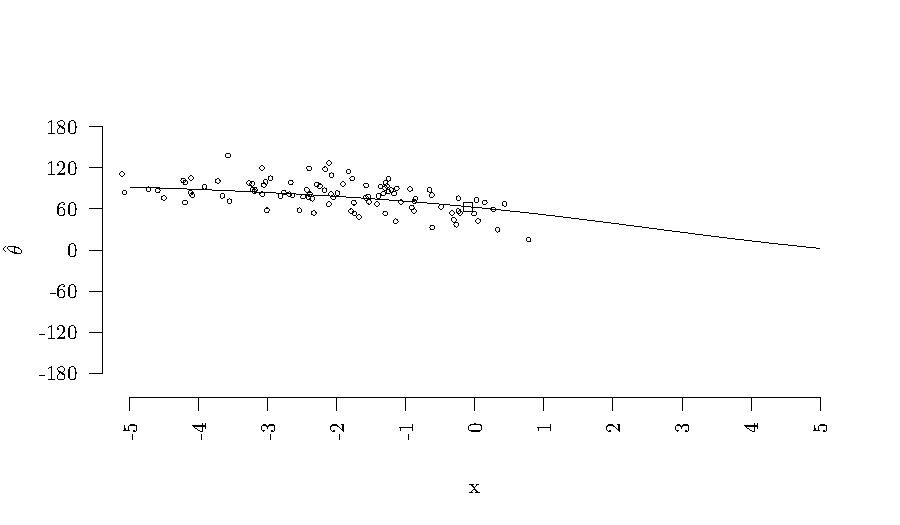
\includegraphics{circregline.pdf}
\caption{Predicted circular regression line for the relation between a linear predictor $x$ and a predicted circular outcome $\theta$ together with the original datapoints. The square indicates the inflection point of the regression line.} 
\label{circregline}
\end{figure}

In Figure \ref{circregline} a circular regression line for the effect of
a predictor \(x\) on the circular outcome is shown. This regression line
can be described using the three circular coefficients \(b_c\), \(SAM\)
and \(AS\). The coefficient \(b_c\) represents the slope of the circular
regression line at the inflection point (the square in Figure
\ref{circregline}). However, this may not be a representative effect for
each dataset as the inflection point can lie in the extremes of the data
(as in Figure \ref{circregline}) or even completely outside the range of
the predictor \(x\). Therefore two additional circular coefficients were
developed by Cremers et al. (2018), \(SAM\) and \(AS\). The coefficient
\(SAM\) represents the slope of the circular regression line at the
average of the predictor \(\bar{x}\) and the coefficients \(AS\)
represents the average slope over all of the predictor values.

\begin{table}
\centering
\caption{Descriptives of the posterior of the coefficients of the effect of L.c on the angular error.} 
\begin{tabular}{lrrrrr}
  \hline\noalign{\smallskip}
Coefficient & mode & mean & sd & LB HPD & UB HPD  \\ \hline\noalign{\smallskip}
$b_c$ & -0.89$^{\circ}$ & -0.21$^{\circ}$ & 1.73$^{\circ}$ & -2.84$^{\circ}$ & 2.55$^{\circ}$\\
$SAM$ &  0.58$^{\circ}$ & -0.84$^{\circ}$ & 90.80$^{\circ}$ & -11.51$^{\circ}$ & 12.73$^{\circ}$   \\
$AS$  & -0.63$^{\circ}$  & -1.11$^{\circ}$  & 92.44$^{\circ}$ & -13.17$^{\circ}$ & 13.14$^{\circ}$ \\
   \hline
\end{tabular}
\label{TableResMapsLc}
\end{table}

For the effect of L.c on the angular error in the cognitive maps data,
the HPD intervals for all three circular coefficients, \(b_c\), \(SAM\)
and \(AS\) include 0 (see Table \ref{TableResMapsLc}. Thus we conclude
that at the inflection point, at the average predictor value and on
average \verb|L.c| the number of training trials does not influence the
angular error. This is in fact a good thing, since it shows that the
training phase of the experiment worked to get all participants at the
same level. For educational purposes we will however continue to give
the interpretation of the coefficients. The \(SAM\) is interpreted as
follows: at the average \verb|L.c|, for a 1 unit increase in \verb|L.c|
the angular error increases with 0.58 degrees. The \(AS\) can be
interpreted as: on average, for a 1 unit increase in \verb|L.c| the
angular error decreases with 0.63 degrees. The \(b_c\) can be
interpreted as: at the inflection point, for a 1 unit increase in
\verb|L.c| the angular error decreases with 0.89 degrees.

\subsubsection{Random Effects}\label{ranme}

In mixed-effects models we are also interested in evaluating the
variance of the random effects. In the model for the cognitive maps data
we included a random intercept. This means that we estimate a separate
intercept for each participant. How to compute random effect variances
on the circle is outlined in Cremers et al. (n.d.). For the cognitive
maps data the posterior mode of the intercept variance on the circle is
estimated at \(3.5*10^{-5}\) and its HPD interval is
\((4.2*10^{-6}; 1.4*10^{-3})\). This variance is very low which means
that the participants do not differ a lot in their individual intercept
estimates. Note that this is not necessarily problematic. In some cases
we are not interested in the variances of the random efects but simply
want to fit a mixed-effects model because we have within factors, such
as \verb|Trial.type|, that cannot be properly incorporated in a standard
regression model.

\subsubsection{Model Comparison}\label{fitme}

When fitting mixed-effects (or multilevel) models we often fit a set of
nested models to our data and follow a model building strategy (Hox,
2002). This can be done top-down, starting with the most complex model,
or bottom-up, starting with the simplest model. Here we use a bottom-up
strategy and start with the so called intercept-only model, a model
containing only a fixed and random intercept:

\begin{Shaded}
\begin{Highlighting}[]
\NormalTok{fit.MapsIO <-}\StringTok{ }\KeywordTok{bpnme}\NormalTok{(}\DataTypeTok{pred.I =}\NormalTok{ Error.rad }\OperatorTok{~}\StringTok{ }\NormalTok{(}\DecValTok{1}\OperatorTok{|}\NormalTok{Subject),}
                    \DataTypeTok{data =}\NormalTok{ Maps,}
                    \DataTypeTok{its =} \DecValTok{10000}\NormalTok{, }\DataTypeTok{burn =} \DecValTok{1000}\NormalTok{, }\DataTypeTok{n.lag =} \DecValTok{3}\NormalTok{, }\DataTypeTok{seed =} \DecValTok{101}\NormalTok{)}
\end{Highlighting}
\end{Shaded}

We then update this model with fixed effects for the predictors at the
lowest level (within-subjects factors), in this case only one,
\verb|Trial.type|. We do this to check whether the set of predictors
improved the fit of the model and can explain a part of the random
intercept variance from the intercept-only model.

\begin{Shaded}
\begin{Highlighting}[]
\NormalTok{fit.Maps1p <-}\StringTok{ }\KeywordTok{bpnme}\NormalTok{(}\DataTypeTok{pred.I =}\NormalTok{ Error.rad }\OperatorTok{~}\StringTok{ }\NormalTok{Trial.type }\OperatorTok{+}\StringTok{ }\NormalTok{(}\DecValTok{1}\OperatorTok{|}\NormalTok{Subject),}
                    \DataTypeTok{data =}\NormalTok{ Maps,}
                    \DataTypeTok{its =} \DecValTok{10000}\NormalTok{, }\DataTypeTok{burn =} \DecValTok{1000}\NormalTok{, }\DataTypeTok{n.lag =} \DecValTok{3}\NormalTok{, }\DataTypeTok{seed =} \DecValTok{101}\NormalTok{)}
\end{Highlighting}
\end{Shaded}

We then add fixed effects for the predictors at the higher level
(between-subjects factors), in this case \verb|Maze| and \verb|L.c|.
Again we do this to check whether they improve the fit of the model and
whether they can explain a part of the random intercept variance.

\begin{Shaded}
\begin{Highlighting}[]
\NormalTok{fit.Maps <-}\StringTok{ }\KeywordTok{bpnme}\NormalTok{(}\DataTypeTok{pred.I =}\NormalTok{ Error.rad }\OperatorTok{~}\StringTok{ }\NormalTok{Maze }\OperatorTok{+}\StringTok{ }\NormalTok{Trial.type }\OperatorTok{+}\StringTok{ }\NormalTok{L.c }\OperatorTok{+}\StringTok{ }\NormalTok{(}\DecValTok{1}\OperatorTok{|}\NormalTok{Subject),}
                  \DataTypeTok{data =}\NormalTok{ Maps,}
                  \DataTypeTok{its =} \DecValTok{10000}\NormalTok{, }\DataTypeTok{burn =} \DecValTok{1000}\NormalTok{, }\DataTypeTok{n.lag =} \DecValTok{3}\NormalTok{, }\DataTypeTok{seed =} \DecValTok{101}\NormalTok{)}
\end{Highlighting}
\end{Shaded}

Because we have already seen that the effect of \verb|L.c| was not
different from 0 we also fit the model with only the \verb|Maze| and
\verb|Trial.type| predictors.

\begin{Shaded}
\begin{Highlighting}[]
\NormalTok{fit.Maps2 <-}\StringTok{ }\KeywordTok{bpnme}\NormalTok{(}\DataTypeTok{pred.I =}\NormalTok{ Error.rad }\OperatorTok{~}\StringTok{ }\NormalTok{Maze }\OperatorTok{+}\StringTok{ }\NormalTok{Trial.type }\OperatorTok{+}\StringTok{ }\NormalTok{(}\DecValTok{1}\OperatorTok{|}\NormalTok{Subject),}
                  \DataTypeTok{data =}\NormalTok{ Maps,}
                  \DataTypeTok{its =} \DecValTok{10000}\NormalTok{, }\DataTypeTok{burn =} \DecValTok{1000}\NormalTok{, }\DataTypeTok{n.lag =} \DecValTok{3}\NormalTok{, }\DataTypeTok{seed =} \DecValTok{101}\NormalTok{)}
\end{Highlighting}
\end{Shaded}

Additional steps, such as adding random slopes for first level
predictors and cross-level interactions, can be taken. In this paper we
will however stick to the previous three models.

\textbf{Model fit}

To assess the fit of the models we look at 4 different model fit
criteria: two version of the deviance information criterion (DIC and
DIC\(_{alt}\)) and two versions of the Watanabe-Akaike information
criterion (WAIC\(_1\) and WAIC\(_2\)) Gelman et al. (2014). We choose
these four criteria because they are specifically useful in Bayesian
models where MCMC methods have been used to estimate the parameters. All
four criteria have a fit part consisting of a measure based on the
loglikelihood and include a penalty in the form of an effective number
of parameters. For all criteria lower values indicate better fit. Gelman
et al. (2014) describes how to compute these criteria. Table
\ref{TableModelFitMaps} shows these criteria for 4 different models.

\begin{table}
\centering
\caption{Model fit criteria for several models fit to the cognitive maps data.} 
\begin{tabular}{lrrrr}
  \hline\noalign{\smallskip}
 Criterion & Intercept-only & \verb|Trial.type| & \verb|Trial.type| + \verb|Maze| & \verb|Trial.type| + \verb|Maze| + \verb|L.c|  \\ \hline\noalign{\smallskip}
DIC             & 304.61 & 267.91 & 253.97 & 257.94 \\
DIC$_{alt}$     & 324.33 & 286.97 & 257.14 & 260.78 \\
WAIC$_1$        & 308.41 & 271.61 & 255.00 & 258.41 \\
WAIC$_2$        & 308.43 & 271.77 & 255.40 & 259.02 \\
   \hline
\end{tabular}
\label{TableModelFitMaps}
\end{table}

In the results for the example we see that the fit improves in all 4
model diagnostics for each model except for the last one. This means
that the predictor \verb|Trial.type| improves the fit of the model over
the intercept-only model and that the predictors \verb|Maze| and
\verb|Trial.type| together improve the fit of the model over the model
with only the \verb|Trial.type| predictor. Because the variable
\verb|L.c| had no effect it is logical that this predictor does not
improve the fit of the most right model over the model with the
\verb|Maze| and \verb|Trial.type| predictors. We conclude that the model
with the predictors \verb|Trial.type| and \verb|Maze| fits best.

\textbf{Explained variance}

Apart from information about whether adding predictors improves the fit
of the model we are also interested in whether these predictors explain
a part of the random effect variances. For the cognitive maps data we
are interested in whether the \verb|Maze| and \verb|Trial.type|
predictors explain a part of the variance in individual intercepts. To
assess this we compare the posterior estimates of the circular random
intercept for the intercept-only model and the model with the
\verb|Maze| and \verb|Trial.type| predictors.

The posterior mode of the intercept variance in the intercept-only model
equals \(6.61*10^{-5} (8.20*10^{-6}; 3.62*10^{-3})\), the posterior mode
of the intercept variance in the model with the \verb|Maze| and
\verb|Trial.type| predictors equals
\(3.25*10^{-5} (4.40*10^{-6}; 1.59*10^{-3})\). First of all, note that
in the intercept-only model there is almost to random intercept
variance. The posterior mode of the circular variance is very close to
0. Compared to the estimates of the variance in the intercept-only model
there is hardly any change in estimates for the variance in the mode
with \verb|Maze| and \verb|Trial.type|.Furthermore, their HPD intervals
have a very large overlap. We thus conclude that the variables
\verb|Maze| and \verb|Trial.type| did not explain any variance in the
random intercepts. This makes sense as there was harly any intercept
variance in the intercept-only model to begin with.

\section{Concluding remarks}\label{conclusion}

In this paper we have given a tutorial for researchers in cognitive
psychology on how to analyse circular data using the package
\verb|bpnreg|. We have covered data inspection in Section
\ref{DataInspection}, the fitting of a Bayesian circular GLM in Section
\ref{RegModel} and the fitting of a Bayesain mixed-effects model in
Section \ref{MEModel}. We have also given a short introduction into the
theoretical background of these models in Section
\ref{EmbeddingApproach} and \ref{embeddingME}.

Apart from the embedding approach to circular data, as used in this
tutorial, there are two other approaches to the analysis of circular
data. In the wrapping approach the data on the circle is assumed to have
origined from wrapping a univariate distribution on the real line onto
the circle. In the intrinsic approach distributions, such as the von
Mises distribution, are directly defined on the circle. For both
approaches models have been described in the literature (Fisher \& Lee,
1992; Gill \& Hangartner, 2010; Lagona, 2016; Mulder \& Klugkist, 2017;
Ravindran \& Ghosh, 2011). The regression model using the intrinsic
approach from Fisher \& Lee (1992) is implemented in the package
\verb|circular| and the circular general linear model from Mulder \&
Klugkist (2017) is implemented in the package \verb|circglmmbayes|. For
neither approach however a detailed tutorial describing how to analyze
circular data using the functions from their package has been written
thus far. Furthermore, the PN approach to circular modelling has the
additional advantage that it is relatively easy to fit more complex
models, e.g.~the mixed-effects model in this tutorial.

\newpage

\hypertarget{references}{%
\section*{References}\label{references}}
\addcontentsline{toc}{section}{References}

\hypertarget{refs}{}
\leavevmode\hypertarget{ref-circularpackage}{}%
Agostinelli, C., \& Lund, U. (2013). \emph{R package \texttt{circular}:
Circular statistics (version 0.4-7)}. Retrieved from
\url{https://r-forge.r-project.org/projects/circular/}

\leavevmode\hypertarget{ref-Batschelet1981}{}%
Batschelet, E. (1981). \emph{Circular statistics in biology}. London:
Academic Press.

\leavevmode\hypertarget{ref-brunye2015map}{}%
Brunyé, T. T., Burte, H., Houck, L. A., \& Taylor, H. A. (2015). The map
in our head is not oriented north: Evidence from a real-world
environment. \emph{PLoS ONE}, \emph{10}(9), 1--12.
doi:\href{https://doi.org/10.1371/journal.pone.0135803}{10.1371/journal.pone.0135803}

\leavevmode\hypertarget{ref-CremersMulderKlugkist2017}{}%
Cremers, J., Mulder, K. T., \& Klugkist, I. (2018). Circular
interpretation of regression coefficients. \emph{British Journal of
Mathematical and Statistical Psychology}, \emph{71}(1), 75--95.
doi:\href{https://doi.org/10.1111/bmsp.12108}{10.1111/bmsp.12108}

\leavevmode\hypertarget{ref-longitudinalpaper}{}%
Cremers, J., Pennings, H. J. M., Mainhard, M. T., \& Klugkist, I.
(n.d.). Longitudinal circular modelling of circumplex measurements for
teacher behavior. \emph{Working Paper}.

\leavevmode\hypertarget{ref-fisher1995statistical}{}%
Fisher, N. I. (1995). \emph{Statistical analysis of circular data}.
Cambridge: Cambridge University Press.

\leavevmode\hypertarget{ref-fisher1992regression}{}%
Fisher, N. I., \& Lee, A. J. (1992). Regression models for an angular
response. \emph{Biometrics}, \emph{48}(3), 665--677.

\leavevmode\hypertarget{ref-BDA}{}%
Gelman, A., Carlin, J., Stern, H., Dunson, D., Vehtari, A., \& Rubin, D.
(2014). \emph{Bayesian data analysis} (3rd ed.). Boca Raton, FL: Chapman
\& Hall/CRC.

\leavevmode\hypertarget{ref-gill2010}{}%
Gill, J., \& Hangartner, D. (2010). Circular data in political science
and how to handle it. \emph{Political Analysis}, \emph{18}(3), 316--336.
doi:\href{https://doi.org/10.1093/pan/mpq009}{10.1093/pan/mpq009}

\leavevmode\hypertarget{ref-heyes2016longitudinal}{}%
Heyes, S. B., Zokaei, N., \& Husain, M. (2016). Longitudinal development
of visual working memory precision in childhood and early adolescence.
\emph{Cognitive Development}, \emph{39}, 36--44.
doi:\href{https://doi.org/10.1016/j.cogdev.2016.03.004}{10.1016/j.cogdev.2016.03.004}

\leavevmode\hypertarget{ref-hox2002multilevel}{}%
Hox, J. J. (2002). \emph{Multilevel analysis: Techniques and
applications}. Hove: Routledge.

\leavevmode\hypertarget{ref-kirschner2009joint}{}%
Kirschner, S., \& Tomasello, M. (2009). Joint drumming: Social context
facilitates synchronization in preschool children. \emph{Journal of
Experimental Child Psychology}, \emph{102}(3), 299--314.
doi:\href{https://doi.org/10.1016/j.jecp.2008.07.005}{10.1016/j.jecp.2008.07.005}

\leavevmode\hypertarget{ref-lagona2016regression}{}%
Lagona, F. (2016). Regression analysis of correlated circular data based
on the multivariate von mises distribution. \emph{Environmental and
Ecological Statistics}, \emph{23}(1), 89--113.
doi:\href{https://doi.org/10.1007/s10651-015-0330-y}{10.1007/s10651-015-0330-y}

\leavevmode\hypertarget{ref-mardia2007protein}{}%
Mardia, K. V., Taylor, C. C., \& Subramaniam, G. K. (2006). Protein
bioinformatics and mixtures of bivariate von mises distributions for
angular data. \emph{Biometrics}, \emph{63}(2), 505--512.
doi:\href{https://doi.org/10.1111/j.1541-0420.2006.00682.x}{10.1111/j.1541-0420.2006.00682.x}

\leavevmode\hypertarget{ref-matsushima2014independence}{}%
Matsushima, E. H., Vaz, A. M., Cazuza, R. A., \& Ribeiro Filho, N. P.
(2014). Independence of egocentric and exocentric direction processing
in visual space. \emph{Psychology \& Neuroscience}, \emph{7}(3),
277--284.
doi:\href{https://doi.org/10.3922/j.psns.2014.050}{10.3922/j.psns.2014.050}

\leavevmode\hypertarget{ref-mulder2017bayesian}{}%
Mulder, K., \& Klugkist, I. (2017). Bayesian estimation and hypothesis
tests for a circular generalized linear model. \emph{Journal of
Mathematical Psychology}, \emph{80}, 4--14.
doi:\href{https://doi.org/10.1016/j.jmp.2017.07.001}{10.1016/j.jmp.2017.07.001}

\leavevmode\hypertarget{ref-nunez2014bayesian}{}%
Nuñez-Antonio, G., \& Gutiérrez-Peña, E. (2014). A Bayesian model for
longitudinal circular data based on the projected normal distribution.
\emph{Computational Statistics \& Data Analysis}, \emph{71}, 506--519.
doi:\href{https://doi.org/10.1016/j.csda.2012.07.025}{10.1016/j.csda.2012.07.025}

\leavevmode\hypertarget{ref-nunez2011bayesian}{}%
Nuñez-Antonio, G., Gutiérrez-Peña, E., \& Escarela, G. (2011). A
Bayesian regression model for circular data based on the projected
normal distribution. \emph{Statistical Modelling}, \emph{11}(3),
185--201.
doi:\href{https://doi.org/10.1177/1471082X1001100301}{10.1177/1471082X1001100301}

\leavevmode\hypertarget{ref-pewsey2013circular}{}%
Pewsey, A., Neuhäuser, M., \& Ruxton, G. D. (2013). \emph{Circular
statistics in r}. Oxford University Press.

\leavevmode\hypertarget{ref-presnell1998projected}{}%
Presnell, B., Morrison, S. P., \& Littell, R. C. (1998). Projected
multivariate linear models for directional data. \emph{Journal of the
American Statistical Association}, \emph{93}(443), 1068--1077.
doi:\href{https://doi.org/10.1080/01621459.1998.10473768}{10.1080/01621459.1998.10473768}

\leavevmode\hypertarget{ref-puglisi2017role}{}%
Puglisi, G., Leonetti, A., Landau, A., Fornia, L., Cerri, G., \&
Borroni, P. (2017). The role of attention in human motor resonance.
\emph{PloS One}, \emph{12}(5), e0177457.
doi:\href{https://doi.org/10.1371/journal.pone.0177457}{10.1371/journal.pone.0177457}

\leavevmode\hypertarget{ref-ravindran2011bayesian}{}%
Ravindran, P., \& Ghosh, S. K. (2011). Bayesian analysis of circular
data using wrapped distributions. \emph{Journal of Statistical Theory
and Practice}, \emph{5}(4), 547--561.
doi:\href{https://doi.org/10.1080/15598608.2011.10483731}{10.1080/15598608.2011.10483731}

\leavevmode\hypertarget{ref-rivest2015general}{}%
Rivest, L.-P., Duchesne, T., Nicosia, A., \& Fortin, D. (2015). A
general angular regression model for the analysis of data on animal
movement in ecology. \emph{Journal of the Royal Statistical Society:
Series C (Applied Statistics)}, \emph{63}(3), 445--463.
doi:\href{https://doi.org/10.1111/rssc.12124}{10.1111/rssc.12124}

\leavevmode\hypertarget{ref-rutishauser2010human}{}%
Rutishauser, U., Ross, I. B., Mamelak, A. N., \& Schuman, E. M. (2010).
Human memory strength is predicted by theta-frequency phase-locking of
single neurons. \emph{Nature}, \emph{464}(7290), 903--907.
doi:\href{https://doi.org/10.1038/nature08860}{10.1038/nature08860}

\leavevmode\hypertarget{ref-warren2017wormholes}{}%
Warren, W. H., Rothman, D. B., Schnapp, B. H., \& Ericson, J. D. (2017).
Wormholes in virtual space: From cognitive maps to cognitive graphs.
\emph{Cognition}, \emph{166}, 152--163.
doi:\href{https://doi.org/10.1016/j.cognition.2017.05.020}{10.1016/j.cognition.2017.05.020}


\end{document}
